\chapter{REMD: GPU ACCELERATION AND EXCHANGES IN MULTIPLE DIMENSIONS}
\label{ch5}

This chapter contains a description of my work implementing replica exchange
molecular dynamics (REMD) in the \emph{pmemd} program of the Amber program
suite. \cite{AMBER12} The first sections describe the general theory of the
state exchanges supported by Amber, followed by details of their implementation.
I'll then finish with a description of my design of multiple-dimension REMD in
Amber that I implemented in both the \emph{sander} and \emph{pmemd} programs.

\section{Temperature REMD}

The most common variant of REMD simulations involves assigning replicas with
different temperatures (T-REMD) \cite{Sugita_ChemPhysLett_1999_v314_p141}
between which the Monte Carlo-based replica exchange attempts occur. The
exchange success probability---calculated in a way that satisfies detailed
balance to preserve valid thermodynamics---is solved for the proposed change of
two replicas swapping temperatures, as shown in Eq. \ref{eq5:TExchProb}.  When
$2N$ replicas are present, $N$ independent exchange attempts can be made
simultaneously between different pairs of replicas. If no replica is involved in
multiple exchange attempts, these moves can be evaluated independently. While
this may not be the most efficient way to perform replica exchange attempts, it
is the most common approach due to its simplicity and efficiency.

To calculate the exchange probability in T-REMD exchange attempts, we start with
the detailed balance equation (Eq. \ref{eq1:DetailedBalance}) in which replicas
$m$ and $n$ have temperatures $T_m$ and $T_n$, respectively in our initial state
$i$. The temperatures swap in our proposed state such that replicas $m$ and $n$
have temperatures $T_n$ and $T_m$, respectively. Because the potential energy
function of each replica is the same---only the temperature differs between
replicas---the probability of a replica having a specific temperature is
directly proportional to the Boltzmann factor (in the canonical ensemble). The
derivation of the exchange probability equation in T-REMD simulations is shown
in Eq. \ref{eq5:TExchProb}.

\begin{align}
   P_{i} \pi_{i \rightarrow j} & = P_{j} \pi_{j \rightarrow i} \nonumber \\
   \frac {\exp \left[ -\beta_m E_m \right] \exp \left[ -\beta_n E_n \right]}
         {Q_m Q_n} \pi_{i \rightarrow j} & = \frac {\exp \left[ -\beta_n E_m
         \right] \exp \left[ -\beta_m E_n \right]} {Q_n Q_m} \pi_{j \rightarrow
         i} \nonumber \\
%  \exp \left[ -\beta_m E_m - \beta_n E_n \right] \pi_{i \rightarrow j} & =
%        \exp \left[ -\beta_n E_m - \beta_m E_n \right] \pi_{j \rightarrow i}
%        \nonumber \\
%  \frac {\pi_{i \rightarrow j}} {\pi_{j \rightarrow i}} & = \frac {\exp \left[
%        -\beta_n E_m - \beta_m E_n \right]} {\exp \left[ -\beta_m E_m - \beta_n
%        E_n \right]} \nonumber \\
%  \frac {\pi_{i \rightarrow j}} {\pi_{j \rightarrow i}} & = \exp \left[
%        -\beta_n E_m - \beta_m E_n + \beta_m E_m + \beta_n E_n \right]
%        \nonumber \\
   \frac {\pi_{i \rightarrow j}} {\pi_{j \rightarrow i}} & = \min \left \lbrace
         1, \exp \left[ (\beta_n - \beta_m) (E_n - E_m) \right] \right \rbrace
   \label{eq5:TExchProb}
\end{align}
where $\beta_m$ is $1/k_BT_m$ for replica $m$ and $E_m$ is the potential energy
of the structure in replica $m$.

Because the temperature of the system uniquely defines its kinetic energy, the
potential energy can be used in lieu of the total energy in Eq.
\ref{eq5:TExchProb} as long as the total temperature remains consistent after
the exchange attempt completes. Therefore, the momenta of replica $m$ are
typically scaled by $\sqrt{T_n/T_m}$ after successfully exchanging with replica
$n$. \cite{Sugita_ChemPhysLett_1999_v314_p141} By scaling the velocities in this
way, snapshots following a successful exchange attempt are immediately
`equilibrated' members of the new temperature's ensemble, thereby eliminating
the need to relax the structure to its `new' temperature. This allows REMD
simulations to be carried out more efficiently by permitting exchange attempts
very frequently. \cite{Sindhikara2008, Sindhikara2010}

An important consideration for T-REMD simulations is how many temperature
replicas you should use as well as what temperatures those replicas should have.
As the temperature of a system increases, the number of low-energy structures
that are sampled during the simulation decreases. In fact, at infinite
temperatures, MD is effectively equivalent to random sampling, whose
consequences were illustrated in Fig. \ref{fig1:EthaneMC}. The temperature
ladder (\ie the selection of temperatures at which to run each replica) should
be chosen so as to optimize the simulation efficiency. If the temperature
difference between adjacent replicas is too great, then the average potential
energy difference between adjacent replicas will be large and the exchange
probability in Eq. \ref{eq5:TExchProb} will be very small. As a result, the low
temperature ensembles will not benefit from the enhanced sampling achievable at
the higher temperatures. On the other hand, if the temperature difference
between adjacent replicas is too small, then computational effort will be wasted
by simulating unnecessary replicas that do not enhance sampling from the
generalized ensemble.

By analyzing Eq. \ref{eq5:TExchProb}, it is clear that in order to have a high
exchange acceptance probability, either the temperature difference or the
potential energy difference between exchanging replicas must be small---in the
extreme case, if a higher temperature replica has a conformation whose potential
energy is less than or equal to the lower-temperature replica, that exchange
attempt is always accepted. By plotting the potential energy distributions
obtained from a short simulation at each temperature, the exchange rate between
any two replicas can be estimated based on the degree by which their potential
energy distributions overlap, shown in Fig. \ref{fig5:TempOverlap}. A good
choice of temperatures for each replica can be made \emph{a priori} based simply
on the number of degrees of freedom present in the system.
\cite{TREMD_Predictor} 

\begin{figure}
   \includegraphics[width=6.5in]{TempOverlap.ps}
   \caption{Potential energy distributions of TrpCage---a 20-residue
            peptide---at various temperatures in a T-REMD simulation.}
   \label{fig5:TempOverlap}
\end{figure}

One challenge with T-REMD is its scalability for large systems. It is well-known
that thermodynamic fluctuations scale as $1/\sqrt{N}$ in statistical ensembles
where $N$ is the total particle count. Therefore, the larger a system gets, the
narrower its potential energy distribution becomes. Consequently, as the
potential energy distributions narrow, replicas must be spaced closer and closer
together to achieve sufficient mixing along the temperature-space parameter. For
this reason, T-REMD simulations on systems that are explicitly solvated are
rare. While some approaches, like the one proposed by \citeauthor{Okur2006}, use
a hybrid solvation scheme whereby exchange attempts are carried out in implicit
solvent, the first two solvation layers are often represented poorly by implicit
solvent, requiring their inclusion even in the hybrid approach. \cite{Okur2006}

Furthermore, the snapshots generated at higher temperatures in the generalized
ensemble are typically discarded from analyses for two reasons. First, we are
typically interested in the thermodynamics of room temperature, so the
high-temperature dynamics are not of general interest. Second, our force fields
are parametrized for use at temperatures near \mbox{300 K}, and higher
temperatures may break the applicability of harmonic functions for several
bonded potentials. While the high-temperature data may be reweighted for
inclusion in low-temperature ensembles,
\cite{Chodera_JChemTheoryComput_2007_v3_p26} higher temperature replicas
contribute increasingly little information to the temperatures of interest.

\section{Hamiltonian REMD}

Another common variant of REMD simulations involves swapping Hamiltonians
between replicas (H-REMD). Because the nature of the exchange in H-REMD
simulations is fundamentally different from those in T-REMD, Eq.
\ref{eq5:TExchProb} cannot be used to calculate the exchange probability for
H-REMD simulations. The proper exchange probability for H-REMD simulations,
generalized for running replicas at different temperatures, is derived in Eq.
\ref{eq5:HExchProb}. Eq. \ref{eq5:HExchProbNotemp} is the special case of Eq.
\ref{eq5:HExchProb} when the temperatures of exchanging replicas are the same.
The easiest and most general way of implementing H-REMD is to swap coordinates
between exchanging replicas. This approach, as implemented in Amber, can be used
for umbrella sampling REMD, \cite{Babin_JChemPhys_2008_v128_p134101,
Sugita_JChemPhys_2000_v113_p6042} accelerated REMD with different boost
parameters, \cite{Fajer_JComputChem_2009_v30_p1719,
Arrar_JChemTheoryComput_2013_v9_p18} and alchemical changes between two end
states. \cite{Meng_JChemTheoryComput_2011_v7_p2721} As a result, Eq.
\ref{eq5:HExchProb} is derived subject to exchanging only coordinates.

\begin{align}
   & P_{i} \pi_{i \rightarrow j} = P_{j} \pi_{j \rightarrow i} \nonumber \\
   & \frac {\exp \left[ -\beta_m H_m(\vec{x}_m) \right] \exp \left[ -\beta_n
         H_n(\vec{x}_n) \right]} {Q_m Q_n} \pi_{i \rightarrow j} = \frac {\exp
         \left[ -\beta_m H_m(\vec{x}_n) \right] \exp \left[ -\beta_n
         H_n(\vec{x}_m) \right]} {Q_n Q_m} \pi_{j \rightarrow i} \nonumber \\
   & \frac {\pi_{i \rightarrow j}} {\pi_{j \rightarrow i}} = \min \left \lbrace
         1, \exp \left[ -\beta_m \left( H_m(\vec{x}_n) - H_m(\vec{x}_m) \right)
         - \beta_n \left( H_n(\vec{x}_m) - H_m(\vec{x}_n) \right) \right] \right
           \rbrace \label{eq5:HExchProb} \\
   & \frac {\pi_{i \rightarrow j}} {\pi_{j \rightarrow i}} = \min \left \lbrace
         1, \exp \left[ -\beta \left( H_m(\vec{x}_n) - H_m(\vec{x}_m) +
         H_n(\vec{x}_m) - H_m(\vec{x}_n) \right) \right] \right \rbrace
   \label{eq5:HExchProbNotemp}
\end{align}

Looking at Eqs. \ref{eq5:HExchProb} and \ref{eq5:HExchProbNotemp}, it is readily
apparent that exchange attempts in H-REMD simulations are far more expensive
than exchange attempts in T-REMD (Eq. \ref{eq5:TExchProb}) or pH-REMD (Eq.
\ref{eq3:ExchSucc}) simulations. To calculate the probability of accepting an
exchange in H-REMD simulations, each replica must calculate the potential energy
of the coordinates of its exchange partner. T-REMD and pH-REMD exchange
probabilities, on the other hand, are calculated via a single exponential of
quantities known \emph{before} the exchange attempt occurs.

When performing replica exchange on an umbrella coordinate, however, the
exchange attempt can be modified to significantly reduce its cost. Since the
underlying Hamiltonian is the same for each replica, the energy differences
$H_m(\vec{x}_n) - H_m(\vec{x}_m)$ are equal to the difference in their umbrella
potentials (Eq. \ref{eq2:umbrella}), which can be calculated very rapidly. This
approach reduces the cost of the exchange attempts in two ways. First, the
umbrella potentials can be swapped between adjacent replicas rather than the
coordinates and momenta, thereby significantly reducing the communication
overhead and eliminating the need to reconstruct a new pairlist immediately.
Second, computing the potential due to an umbrella restraint requires a small
number of geometric measurements, which is negligible compared to evaluating the
energy of the entire system (including the restraint potential).

Despite the apparently high cost of evaluating Eq. \ref{eq5:HExchProb},
attempting exchanges every 100 MD steps incurs, at most, a 1\% performance hit
due to performing one extra energy evaluation every 100 steps (each of which
requires a full force evaluation for standard dynamics). Therefore, there has
not been enough incentive for writing an optimized exchange routine specifically
for umbrella sampling simulations in Amber. Such an exchange routine would be
useful in future studies if Gibbs' sampling exchange attempts were implemented,
\cite{Chodera_JChemPhys_2011_v135_p194110} or in situations where swapping only
an umbrella potential simplifies calculating Eq. \ref{eq5:HExchProb}.

\paragraph{Replica Exchange Free Energy Perturbation}

Here I will refocus on free energy perturbation---Eq.  \ref{eq2:FEP}---and its
relationship with the H-REMD exchange probability shown in Eq.
\ref{eq5:HExchProbNotemp}. By comparing these two equations, we see that the
energy differences required in Eq. \ref{eq2:FEP} are calculated every time the
exchange probability is calculated in Eq. \ref{eq5:HExchProbNotemp}!  Therefore,
the term $\left\langle\exp\left(-\beta(E_B-E_A))\right)\right\rangle$ can be
accumulated in both the forward and reverse directions during the course of the
H-REMD simulation. This approach of computing FEP-based energy differences
between two states during a H-REMD simulation is referred to as \emph{Replica
Exchange Free Energy Perturbation} (REFEP).
\cite{Meng_JChemTheoryComput_2011_v7_p2721,
Jiang_JChemTheoryComput_2010_v6_p2559}

\section{Multi-Dimensional REMD}

As the architecture of modern computers continues its push into massive
parallelization, highly scalable techniques such as REMD become increasingly
cost-efficient methods in the field of computational chemistry. While we have
seen that REMD simulations, in general, enhance sampling by expanding our
original ensemble though state space (\eg temperature space, Hamiltonian space,
etc.), different variants of REMD bestow different advantages on the simulation.
For instance, T-REMD enhances conformational sampling by flattening the free
energy surface, pH-REMD enhances sampling by allowing simulations to dodge free
energy barriers through pH-space, and H-REMD enhances conformational sampling by
coupling different energy functions.

As availability to large numbers of processing cores increases, it becomes
feasible to combine multiple types of replica exchanges into a single,
super-expanded ensemble. In this new, larger ensemble, replicas are defined by a
series of state parameters, such as a specific temperature, Hamiltonian,
umbrella potential, or solution pH. Exchange attempts between replicas must now
take into account changes in multiple state parameters, which may lead to
complex equations for the exchange probability. To simplify the exchange
process, the replicas can be separated into different \emph{dimensions} in which
only a single state variable changes along that dimension.

By adopting this approach, the exchange routines described in previous chapters
and sections can be reused in this new, multi-dimensional REMD method. To
visualize which exchanges are performed, consider a 2-dimensional square matrix
in which the rows and columns represent two different state parameters. In
single rows or columns, only a single state parameter changes, so the exchange
probability equations that have already been derived apply to these exchange
attempts. Fig. \ref{fig5:MultiDREMD} displays the arrangement of replicas---and
the allowed exchange attempts---in a simple diagram. While these ideas can be
trivially extended to an arbitrary number of dimensions, the number of replicas
required increases exponentially with each additional dimension.

\begin{figure}
   \includegraphics[height=6.5in, angle=90]{MultiDREMD.ps}
   \caption{Schematic showing exchange attempts in multi-dimensional REMD
            simulations. Exchange attempts are indicated by the colored arrows,
            where red arrows indicate exchange attempts between the \emph{j}
            state parameters and blue arrows indicate exchange attempts between
            the \emph{i} state parameters}
   \label{fig5:MultiDREMD}
\end{figure}

\section{Implementation}

In this section, I will describe how REMD is implemented in Amber, with focus
paid to how exchange attempts are carried out as well as the programmatic
details of how information is traded between exchanging replicas.

\subsection{Exchange Attempts}

Specific details of how and when exchanges are attempted between replicas is
very important to not only the efficiency of our overall simulations, but also
the theoretical rigor of its correctness. As I have already mentioned, exchange
attempts are restricted to a single pair of replicas in which only a single
state parameter differs between them. The question of \emph{which} replicas
attempt to exchange information also has a strong impact on how quickly
observable properties converge. The easiest and most na\"ive approach is to
choose a single partner and attempt an exchange. To maximize the likelihood that
the exchange attempt is successful, exchanges are attempted between
nearest-neighbors in the state parameter that is being swapped. Due to its
simplicity, this is the approach that was implemented in Amber by
\citeauthor{Cheng2005}. \cite{Cheng2005} Recent evidence suggests, however, that
such an approach limits sampling in the state space coordinate.
\cite{Chodera_JChemPhys_2011_v135_p194110} Sampling along the state space
coordinate can be enhanced by employing ideas from \emph{Gibbs' sampling},
\cite{Chodera_JChemPhys_2011_v135_p194110} or simply increasing the frequency
of exchange attempts. \cite{Sindhikara2008, Sindhikara2010}

Another important consideration in REMD simulations is \emph{when} to suspend
the MD in each dimension and attempt to exchange information. Strict adherence
to the condition of detailed balance and the principle of reversibility in the
resulting chain of states requires these exchange attempts be done
stochastically. \cite{Chodera_JChemPhys_2011_v135_p194110} However, while
deterministic exchange attempts violate detailed balance, they satisfy the less
restrictive condition of general balance, so the thermodynamical rigor of such
an approach is preserved. \cite{Chodera_JChemPhys_2011_v135_p194110} Amber
employs a deterministic, synchronous approach to deciding when exchange attempts
should be performed by attempting exchanges between adjacent replicas every $n$
steps, where $n$ is a tunable input parameter.

Also important is the nature of the exchange itself. The two approaches
currently used in Amber---exchanging state parameters or exchanging
coordinates---are described below.

\paragraph{Exchanging State Parameters}

The most efficient way to carry out replica exchanges is to swap state
parameters---an approach used in Amber for both T-REMD and pH-REMD. In this
case, replicas typically differ by a term that modifies a potential energy
function that is otherwise the same for each replica. In this instance,
simulations are subject to a different thermodynamic constraint after exchanges
are successful. Following successful exchanges, the position of each replica in
the ordered list of state parameters changes. As a result, the nearest neighbors
between whom exchanges are attempted changes after each exchange attempt.
Prior to each exchange attempt, each replica must figure out where every replica
resides in state space so they know how to carry out exchanges.

When exchanging state parameters, replicas typically need to exchange a minimal
amount of information---their state parameter and a related conjugate property.
In the case of T-REMD, replicas exchange temperatures and potential energies,
and individual replicas adopt different temperatures as a function of time. For
pH-REMD, the solution pH and total number of `active' titratable protons are
swapped between adjacent replicas.

When an exchange attempt can be completed simply by swapping states, the
resulting output files from the simulations follow the course of a single
trajectory as it passes through both phase space and state space. As a result,
the trajectory file must be modified so that the state parameter of each frame
can be identified. This is necessary for reconstructing the sub-ensemble of
interest (\eg the ensemble at 300 K, or pH 7). While this approach adds the
complexity of the bookkeeping required to post-process the data, the
communication required scales as $O(1)$ with system size, improving the
scalability of these REMD simulations.
\cite{Swails_JChemTheoryComput_2012_v8_p4393} Because the cost of exchange
attempts in this family of REMD methods is negligible, there is no practical
limit to the frequency with which replicas attempt to exchange, allowing us to
take advantage of the faster convergence accessible via rapid exchange attempts
\cite{Sindhikara2008, Sindhikara2010} or Gibbs' sampling.
\cite{Chodera_JChemPhys_2011_v135_p194110}

\paragraph{Exchanging Coordinates and Momenta}

The alternative to swapping state parameters between replicas is to swap
coordinates and their conjugate momenta, which is logically equivalent to
swapping full potential energy functions. It is significantly simpler---and
requires far less communication between exchanging replicas to be fully
general---than swapping the full potential energy function. It is for the added
simplicity and reduced communication overhead that H-REMD is implemented in
Amber by swapping coordinates and velocities (scaling the velocities if
exchanging pairs have different temperatures).
\cite{Meng_JChemTheoryComput_2011_v7_p2721}

Adding to the computational expense, however, is the need to either recompute or
exchange the full pairlist of each replica. Either choice is quite expensive
since the pairlist is a very large array that requires evaluating all pairwise
distances in the system to build. Unlike approaches that exchange state
parameters, the cost of exchange attempts that require coordinate exchanges and
extra energy evaluations (and multiple additional pairlist builds) imposes a
very real upper limit on the practical efficiency of employing rapid exchange
attempts or Gibbs' sampling ideas to these simulations.

The most efficient way of performing REMD using umbrella potentials would be to
swap the umbrella potentials---essentially a state parameter---and track a
replica's trajectory through umbrella space.

\subsection{Message Passing: Data Exchange in REMD Simulations}

While REMD simulations can be carried out `in serial' by simulating chunks of
each replica sequentially by a single process, such an approach defeats the
purpose of proposing REMD simulations as a scalable protocol for enhanced
sampling. REMD is most efficient when each replica can be simulated
simultaneously using different processes, or \emph{threads}. The main simulation
engines in Amber use the \emph{Message Passing Interface} (MPI) to enable
distributed memory parallelization (\ie each working thread contains its own
memory that is inaccessible by other threads). MPI---described in more detail in
Appendix \ref{appendixC}---is ideally suited for large-scale parallelization
since it allows workers to be spread across multiple processing cores that do
not share a common memory bank. The most powerful supercomputers in the world
that we typically use to carry out our simulations are so-called
\emph{distributed} supercomputers since they are constructed from many
individual computers with dedicated memory that are networked together.

MPI enables parallelism by allowing groups of threads to exchange information by
sending and receiving data through a series of predefined functions and
subroutines (typically called an application programmer interface, or API).
Data, or \emph{messages}, can be sent and received between two threads in an MPI
program that are grouped together in the same \emph{communicator}. Because
communicators provide a simple and efficient way of programmatically separating
threads into different groups, we take advantage of this feature when organizing
the workload in MPI programs. Intra-replica communication---which allows a
single replica to be run using multiple processors---is handled by a dedicated
replica communicator. The arbitrarily designated `first' thread---or
\emph{master}---of all replicas are assigned to separate communicators for
sending all data pertinent to carrying out replica exchange attempts.

In typical REMD simulations involving only a single state parameter, the REMD
communicator is simply a communicator that links all replica masters. In
multi-dimensional REMD, however, exchanges are only permitted between replicas
that differ in only one state parameter. Therefore, communicators are defined
between only those replicas between which exchanges are permitted. Using Fig.
\ref{fig5:MultiDREMD} as a guide, communicators are defined between the masters
of the replicas in a single row or column. These communicators have to be set up
and destroyed after each exchange attempt because successful exchange attempts
in a dimension that implements state parameter swaps will change the REMD
communicator that the replica belongs to in the other dimensions. This is
illustrated in Fig. \ref{fig5:MultiDREMDExchg}.

\begin{figure}
   \includegraphics[height=6.5in, angle=90]{MultiDREMDExchg.ps}
   \caption{Communicator arrangement in multi-dimensional REMD simulations at
            multiple exchange steps following some successful state parameter
            exchanges. The large numbers in the background are the (unchanging)
            thread numbers in the communicator linking the `master' threads of
            each replica. The blue and red numbers are the indexes in the first
            and second state parameter tables, respectively. Every cell with the
            same background color is a member of the same REMD communicator.}
   \label{fig5:MultiDREMDExchg}
\end{figure}
